\section{Lựa chọn OPAMP sử dụng, mô phỏng OPAMP theo datasheet}

\subsection{Mạch tạo nguồn dòng}

Với yêu cầu tạo một mạch cho ngõ ra một nguồn dòng ổn định theo nhiệt độ ở giá trị $I_{const} = 1\,\textsf{mA}$, ta có mạch tạo nguồn dòng như sau:

\begin{figure}[H]
	\centering
	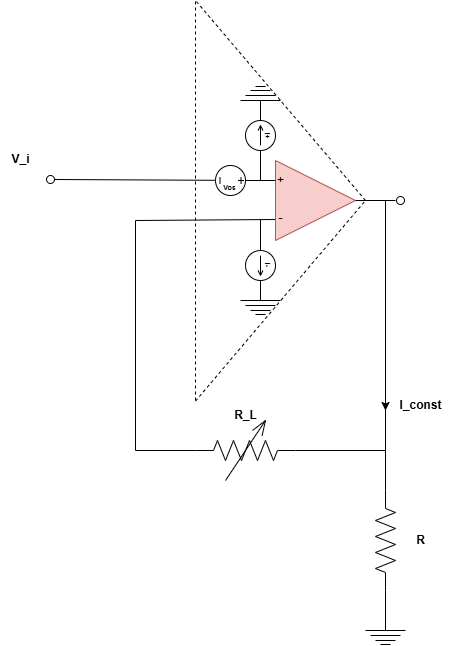
\includegraphics[width=.4\linewidth]{./my-chapters/my-diagrams/current_const.png}
\end{figure}

Với công thức của mạch trên là: $I_{const} = \dfrac{V_{i}}{R_{1}} \pm \dfrac{V_{os}}{R_{1}} \mp I_{-}$

Ta có, $V_{i} = 1\,\textsf{V}$ và $R_{1} = 1\,\textsf{k}\Omega$ để cho ra được ngõ ra $I_{const} = \dfrac{1}{1\,\textsf{k}} = 1\,\textsf{mA}$. Vậy để sai số không ảnh hưởng quá nhiều vào mạch thì $\pm \dfrac{V_{os}}{R_{1}} \mp I_{-} << 1\,\textsf{mA}$ để không ảnh hưởng quá nhiều vào dòng điện ngõ ra.

\begin{enumerate}[label=\arabic*.]
	\item Chọn $V_{os}$:
	\[ \left | \dfrac{V_{os}}{R_{1}} \right |  < 0.01\,\textsf{mA} \Rightarrow V_{os} < 10\,\textsf{mV}\]
	\item Chọn $I_{ib}$ và $I_{os}$:
	\[ I_{-} < 0.1\,\textsf{mA} \Rightarrow 
	\left\{ 
		\begin{matrix}
			I_{os} = | I_{+} - I_{-} | < 1\,\mu\textsf{A}\\[6pt]
			I_{ib} = \dfrac{I_{+} + I_{-}}{2} < 1\,\mu\textsf{A} 
		\end{matrix}	
	\right. 
	\]
\end{enumerate}

Nhóm em chọn OPAMP \href{https://file.thegioiic.com/upload/documents/1740470713_CA3140E.pdf}{CA3140E} với các thông số như sau:

\begin{figure}[H]
	\centering
	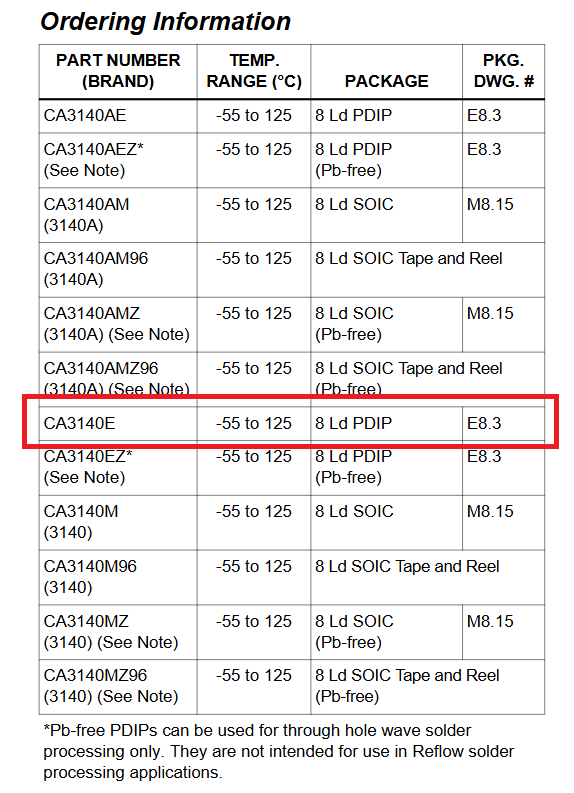
\includegraphics[width=0.7\linewidth]{my-chapters/my-images/Sel_OPAMP/CA3140E_current_const.png}
	\caption{Tầm nhiệt độ có thể hoạt động.}
\end{figure}

\begin{figure}[H]
	\centering
	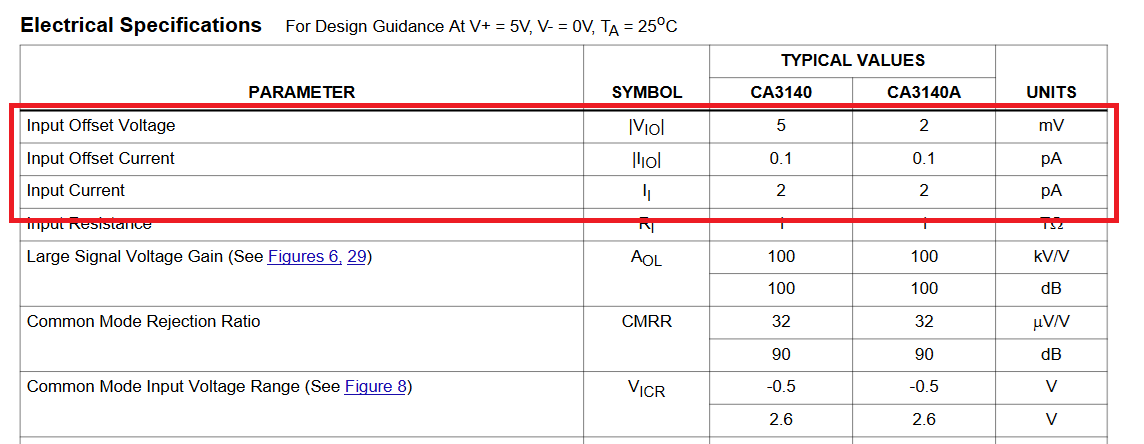
\includegraphics[width=0.7\linewidth]{my-chapters/my-images/Sel_OPAMP/CA3140E_offset.png}
	\caption{Các sai số Offset của OPAMP.}
\end{figure}

\begin{figure}[H]
	\centering
	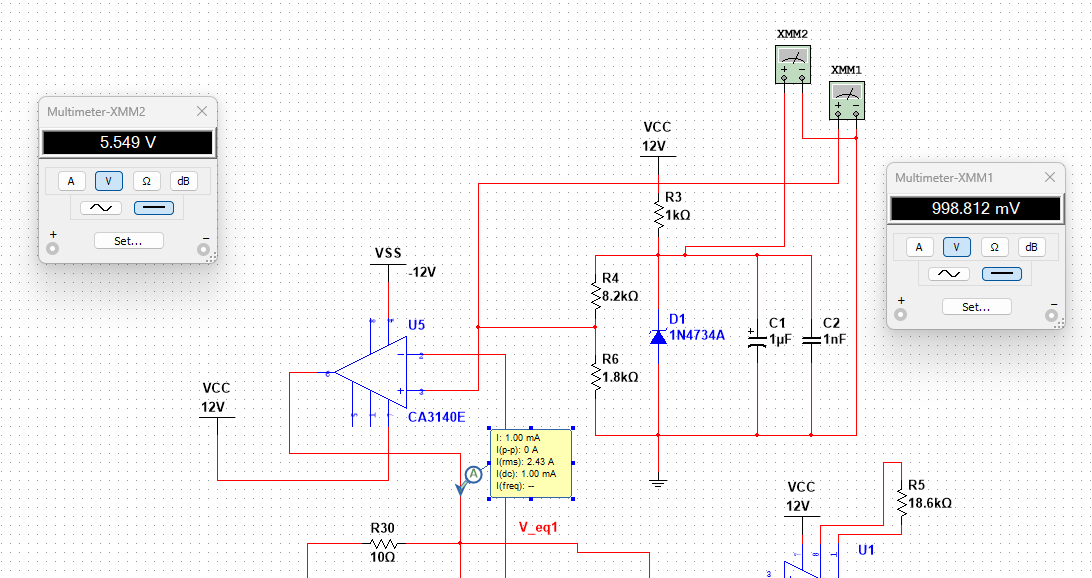
\includegraphics[width=0.7\linewidth]{my-chapters/my-images/Sel_OPAMP/CA3140E_I_circuit.png}
	\caption{Mạch mô phỏng nguồn dòng ở trạng thái không lý tưởng.}
\end{figure}

\begin{figure}[H]
	\centering
	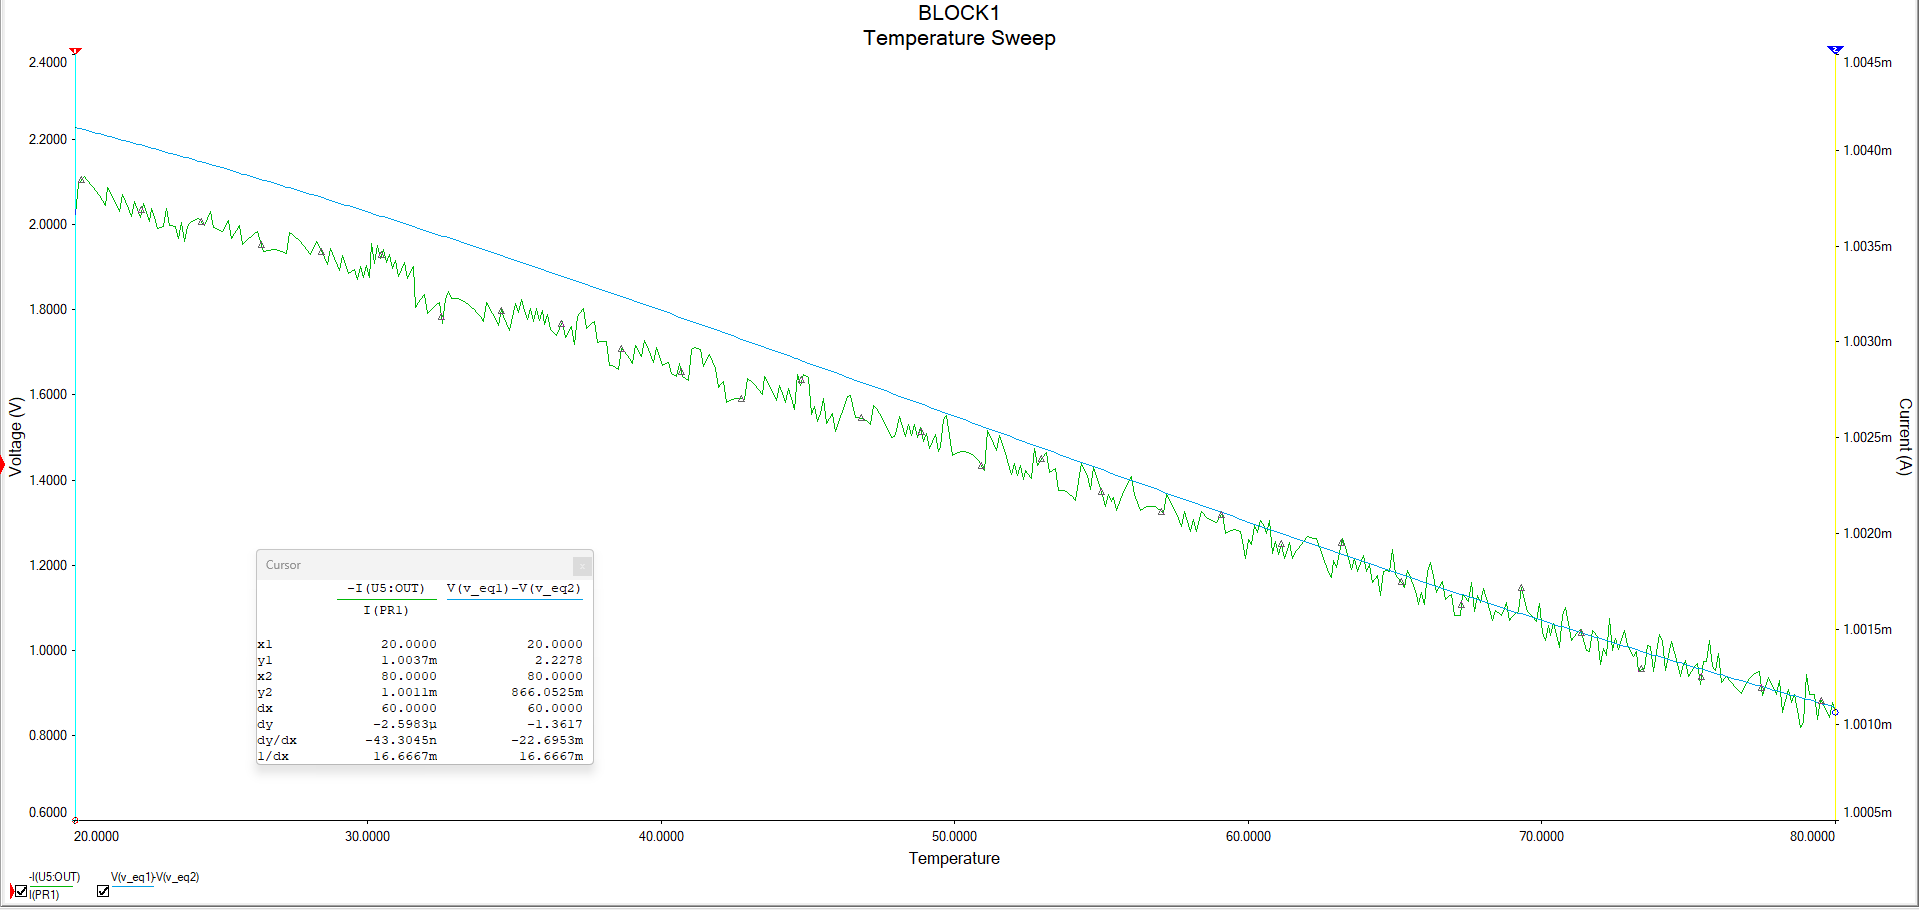
\includegraphics[width=0.7\linewidth]{my-chapters/my-images/Sel_OPAMP/CA3140E_I_sim_1.png}
	\caption{Mô phỏng giá trị $V_{eq1} - V_{eq2}$ với nguồn dòng không lý tưởng.}
	\label{fig:ca3140eisim1}
\end{figure}

\subsection{Mạch khuếch đại vi sai}

Mạch thực hiện chức năng khuếch đại vi sai ở Tầng 2 như sau:

\begin{figure}[H]
	\centering
	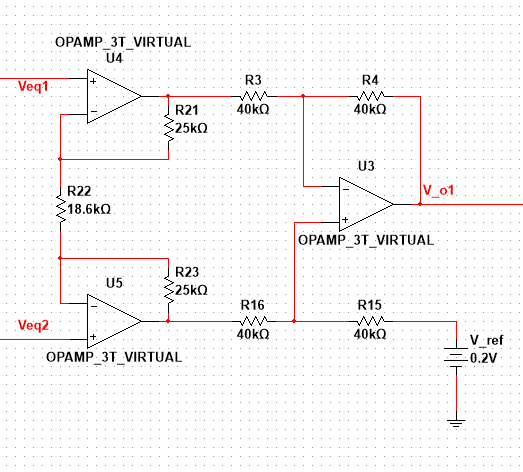
\includegraphics[width=.8\linewidth]{./my-chapters/my-images/Sel_OPAMP/INA128PA_schematic_ideal.png}
\end{figure}

Theo như mạch trên có cấu trúc của con \href{https://www.ti.com/lit/ds/symlink/ina128.pdf?ts=1764428509260&ref_url=https%253A%252F%252Fwww.ti.com%252Fproduct%252FINA128%253Futm_source%253Dgoogle%2526utm_medium%253Dcpc%2526utm_campaign%253Dasc-null-null-GPN_EN-cpc-pf-google-soas_en_cons%2526utm_content%253DINA128%2526ds_k%253DINA128+Datasheet%2526DCM%253Dyes%2526gclsrc%253Daw.ds%2526gad_source%253D1%2526gad_campaignid%253D8754035891%2526gbraid%253D0AAAAAC068F13fbuMaTyj24n6YvykwekOe%2526gclid%253DCj0KCQiA0KrJBhCOARIsAGIy9wA-sSmwQ7GAyqSI0TxGaZzATEH10kYNY7CLkiZxrrshCKCRgCthqHoaAt7cEALw_wcB}{INA128} có cấu trúc như sau:

\begin{figure}[H]
	\centering
	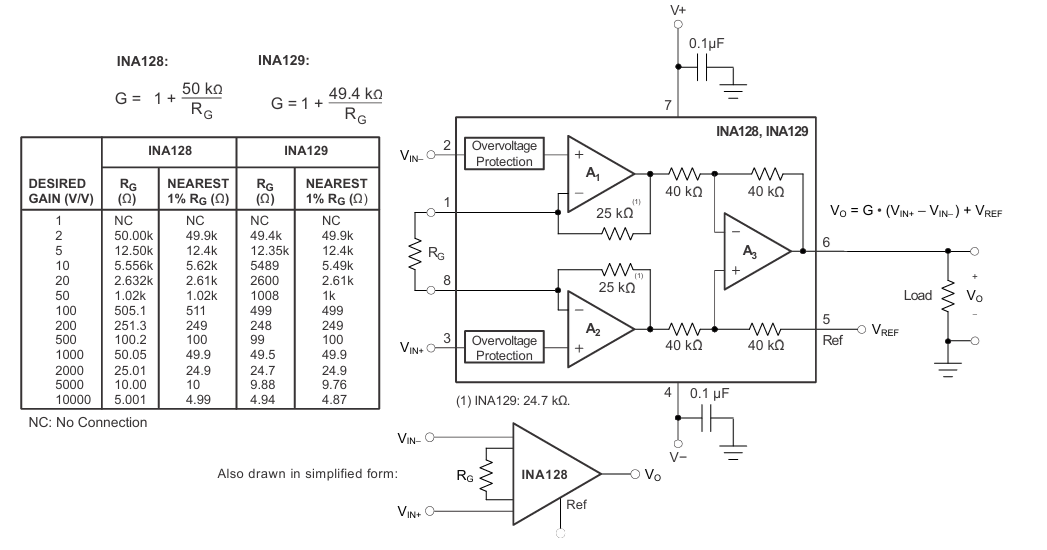
\includegraphics[width=.9\linewidth]{./my-chapters/my-images/Sel_OPAMP/INA128_overview.png}
	\caption{Sơ đồ tổng quan và công thức tính của INA128.}
\end{figure}

Ta thực hiện một căn chỉnh $V_{ref} = 0.2\,\textsf{V}$ như sau:

\begin{figure}[H]
	\centering
	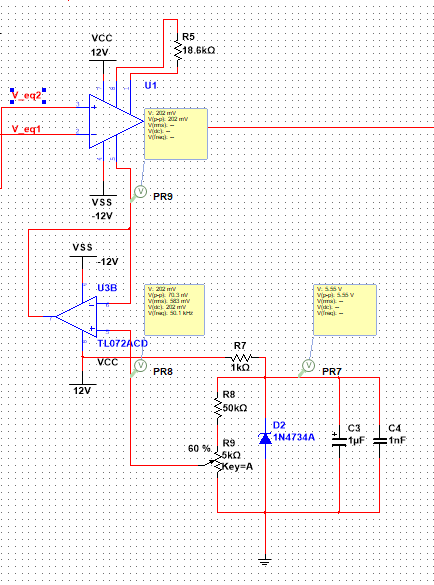
\includegraphics[width=.7\linewidth]{./my-chapters/my-images/Sel_OPAMP/INA128_Vref.png}
	\caption{Mạch căn chỉnh $V_{ref}$ cho INA128.}
\end{figure}

\subsection{Mạch cộng điện áp}

Ta xét ở tầng khuếch đại:

\begin{figure}[H]
	\centering
	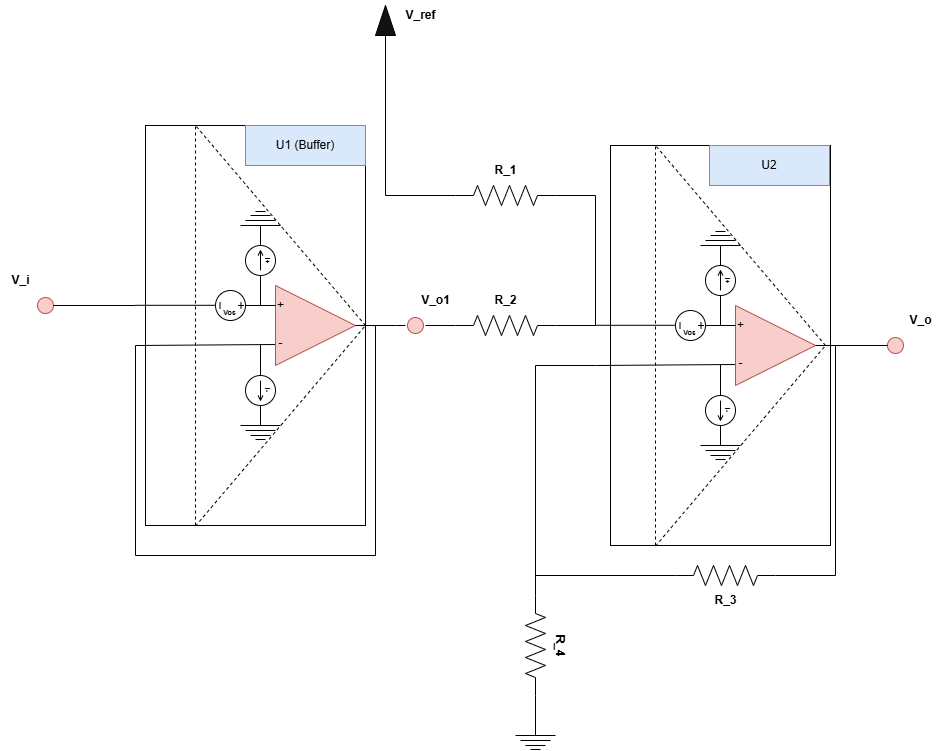
\includegraphics[width=.7\linewidth]{./my-chapters/my-diagrams/Stage_Amplifier.png}
\end{figure}

\begin{enumerate}[label=\arabic*.]
	\item Xét tại OPAMP đầu tiên có chức năng là một Buffer:
	
	\[ V_{o1} = V_{i} \pm V_{os} \]
	
	\item Xét tại OPAMP thứ hai có chức năng là thực hiện hàm $V_{o} = V_{i} + V_{ref}$:
	
	\[ V_{o} = \left( 1 + \dfrac{R_{3}}{R_{4}} \right)\left( V_{ref}\dfrac{R_{2}}{R_{1} + R_{2}} + V_{o1}\dfrac{R_{1}}{R_{1} + R_{2}} \right) \pm V_{os}\left( 1 + \dfrac{R_{3}}{R_{4}} \right) \mp I_{-}R_{3} \]
\end{enumerate}

Chọn $R_{1} = R_{2} = 1\,\textsf{k}\Omega$

Chọn $R_{3} = R_{4} = 1\,\textsf{k}\Omega$

Ta xét 2 con OPAMP trên là cùng một Package, ta có:

\begin{enumerate}[label=\arabic*.]
	\item Xét tại OPAMP đầu tiên có chức năng là một Buffer với ngõ điện áp ngõ ra sai số 5\% giá trị thì tại đây nhóm em chọn sai số phải rơi vào dưới 1\%:
	
	\[ \pm V_{os} < 0.08\,\textsf{V}\]
	$\Rightarrow V_{os} $ phải có giá trị ở dưới 10 lần ngưỡng trên là cỡ $8\,\textsf{mV}$.
	\item Xét tại OPAMP thứ hai phải có ngõ ra cũng rơi vào dưới 1\%:
	
	\[ \pm V_{os}\left( 1 + \dfrac{R_{3}}{R_{4}} \right) \mp I_{-}R_{3} < 0.05\,\textsf{V} \]
	$\Rightarrow$ Với $V_{os} < 10\,\textsf{mV}$ thì $I_{-} > 70\,\mu\textsf{A}$.
	
	$\Rightarrow \left\{ 
		\begin{matrix}
			I_{os} = | I_{+} - I_{-} | < 30\,\mu\textsf{A}\\[6pt]
			I_{ib} = \dfrac{I_{+} + I_{-}}{2} < 15\,\mu\textsf{A} 
		\end{matrix}
	\right.$
\end{enumerate}

Từ đó ở tầng khuếch đại nhóm em sử dụng \href{https://file.thegioiic.com/upload/documents/1740471008_LMV358IDGKR.pdf}{LMV358IDGKR}, với thông số sau:

\begin{figure}[H]
	\centering
	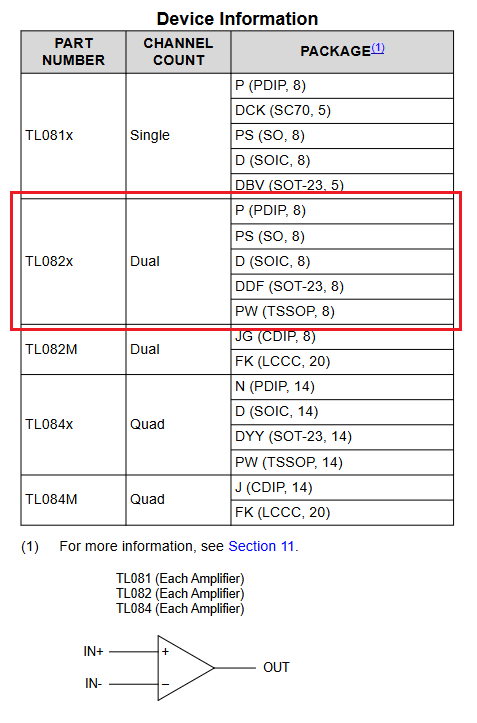
\includegraphics[width=.4\linewidth]{./my-chapters/my-images/Sel_OPAMP/TL082_package.png}
\end{figure}

\begin{figure}[H]
	\centering
	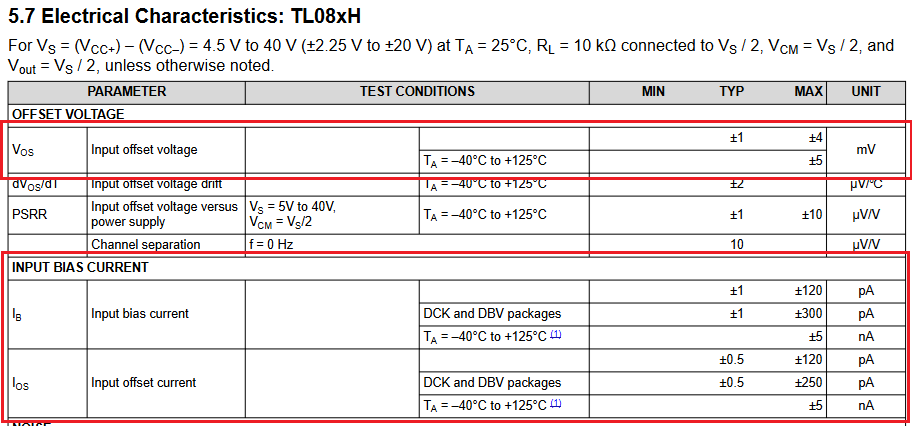
\includegraphics[width=.8\linewidth]{./my-chapters/my-images/Sel_OPAMP/TL08_vos_iib_ios.png}
\end{figure}

\subsection{Mạch tổng quát}

\begin{figure}[H]
	\centering
	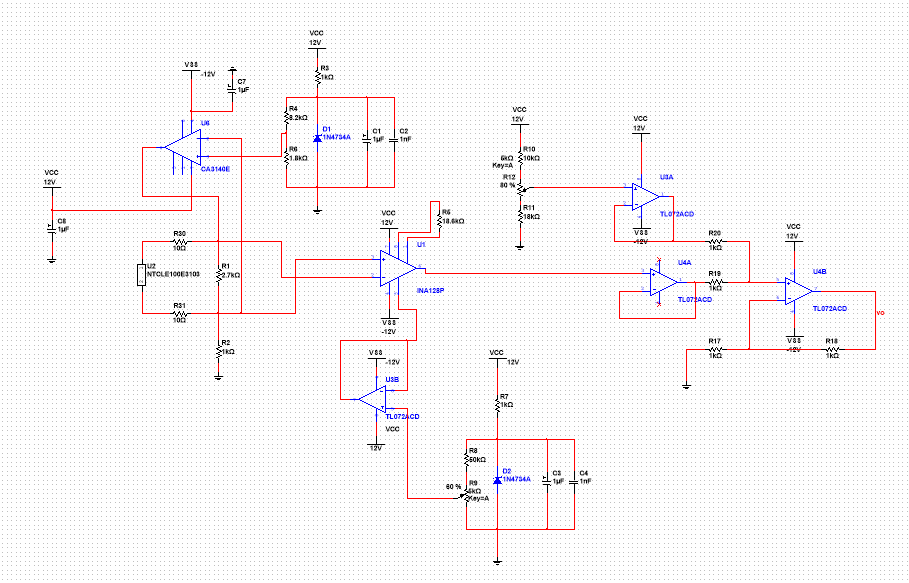
\includegraphics[width=\linewidth]{./my-chapters/my-images/schematic_tongthe.png}
	\caption{Thiết kế mạch tổng quát của mạch đo nhiệt độ từ Sensor NTCLE100E3.}
\end{figure}

\begin{figure}[H]
	\centering
	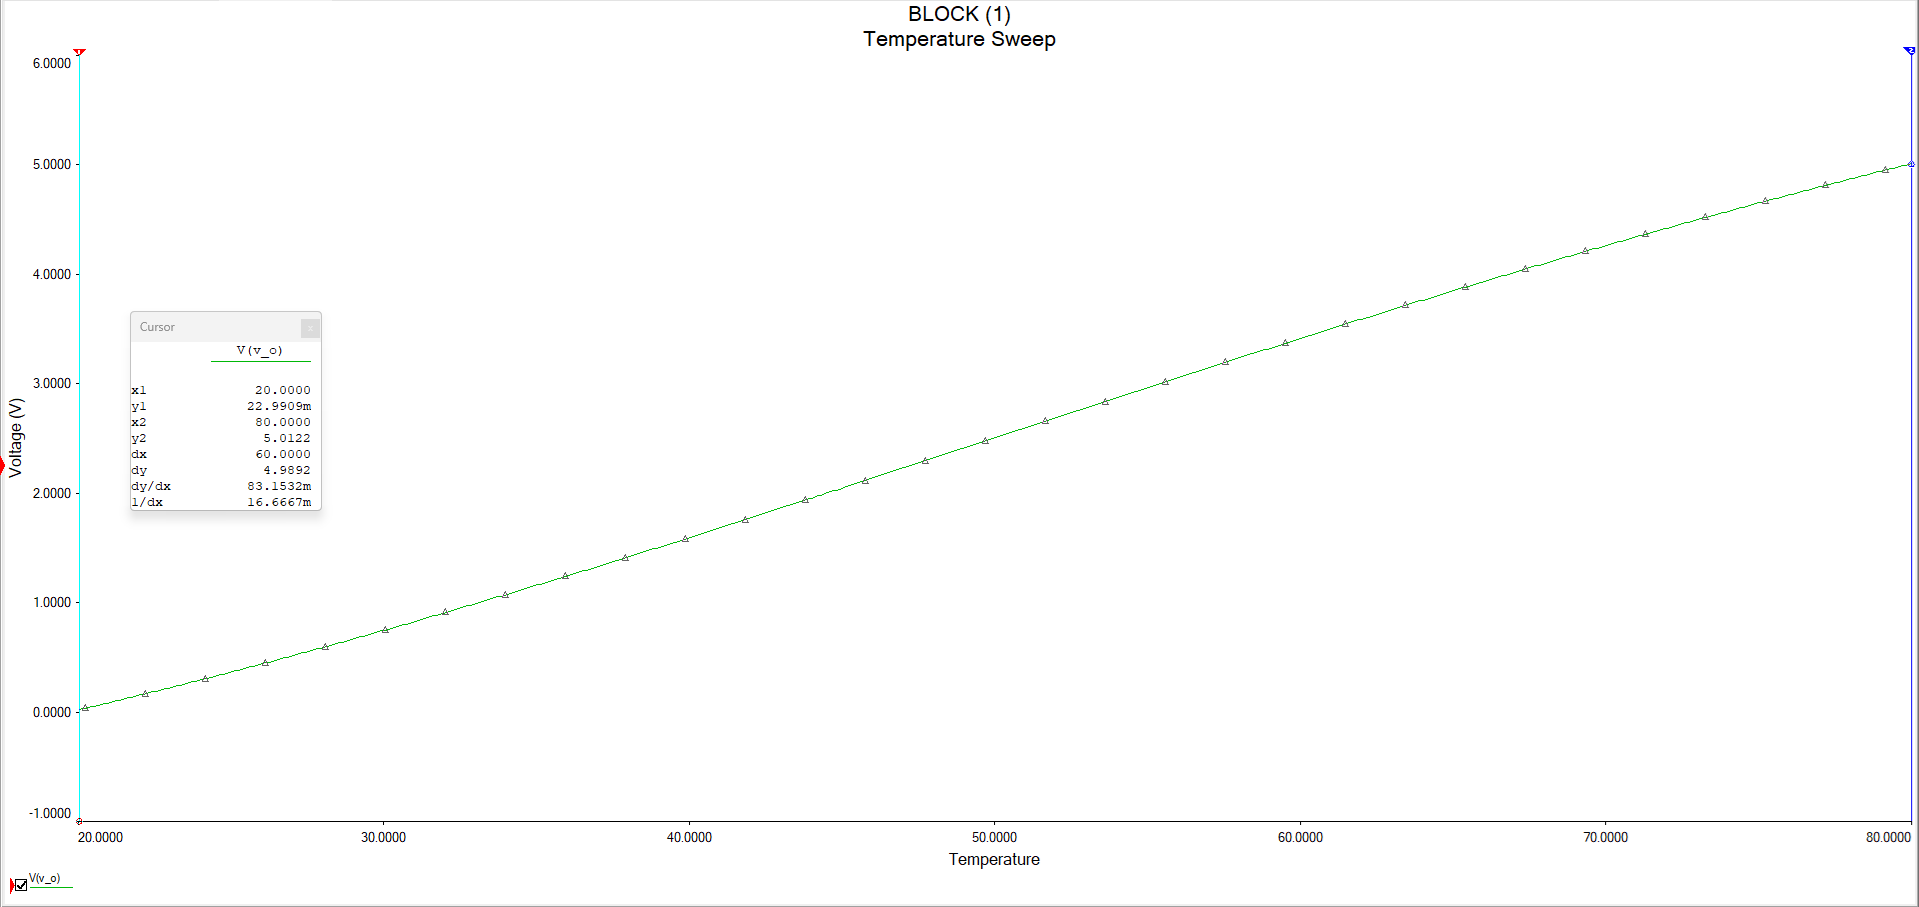
\includegraphics[width=.9\linewidth]{./my-chapters/my-images/OutPut_V_final.png}
	\caption{Kết quả sau khi chạy mô phỏng đo từ $20\rightarrow80^{o}C$ bằng Sensor NTCE100E3.}
\end{figure}

Sau đây là bảng Excel tính giá trị của mạch:

\begin{itemize}[label=-]
	\item Giá trị sai số lớn nhất là: \finalresult{Max\_Error = 3.4168\%}.
	\item Giá trị sai số nhỏ nhất là: \finalresult{Min\_Error = 0.0004\%}.
\end{itemize}

\begin{landscape}
	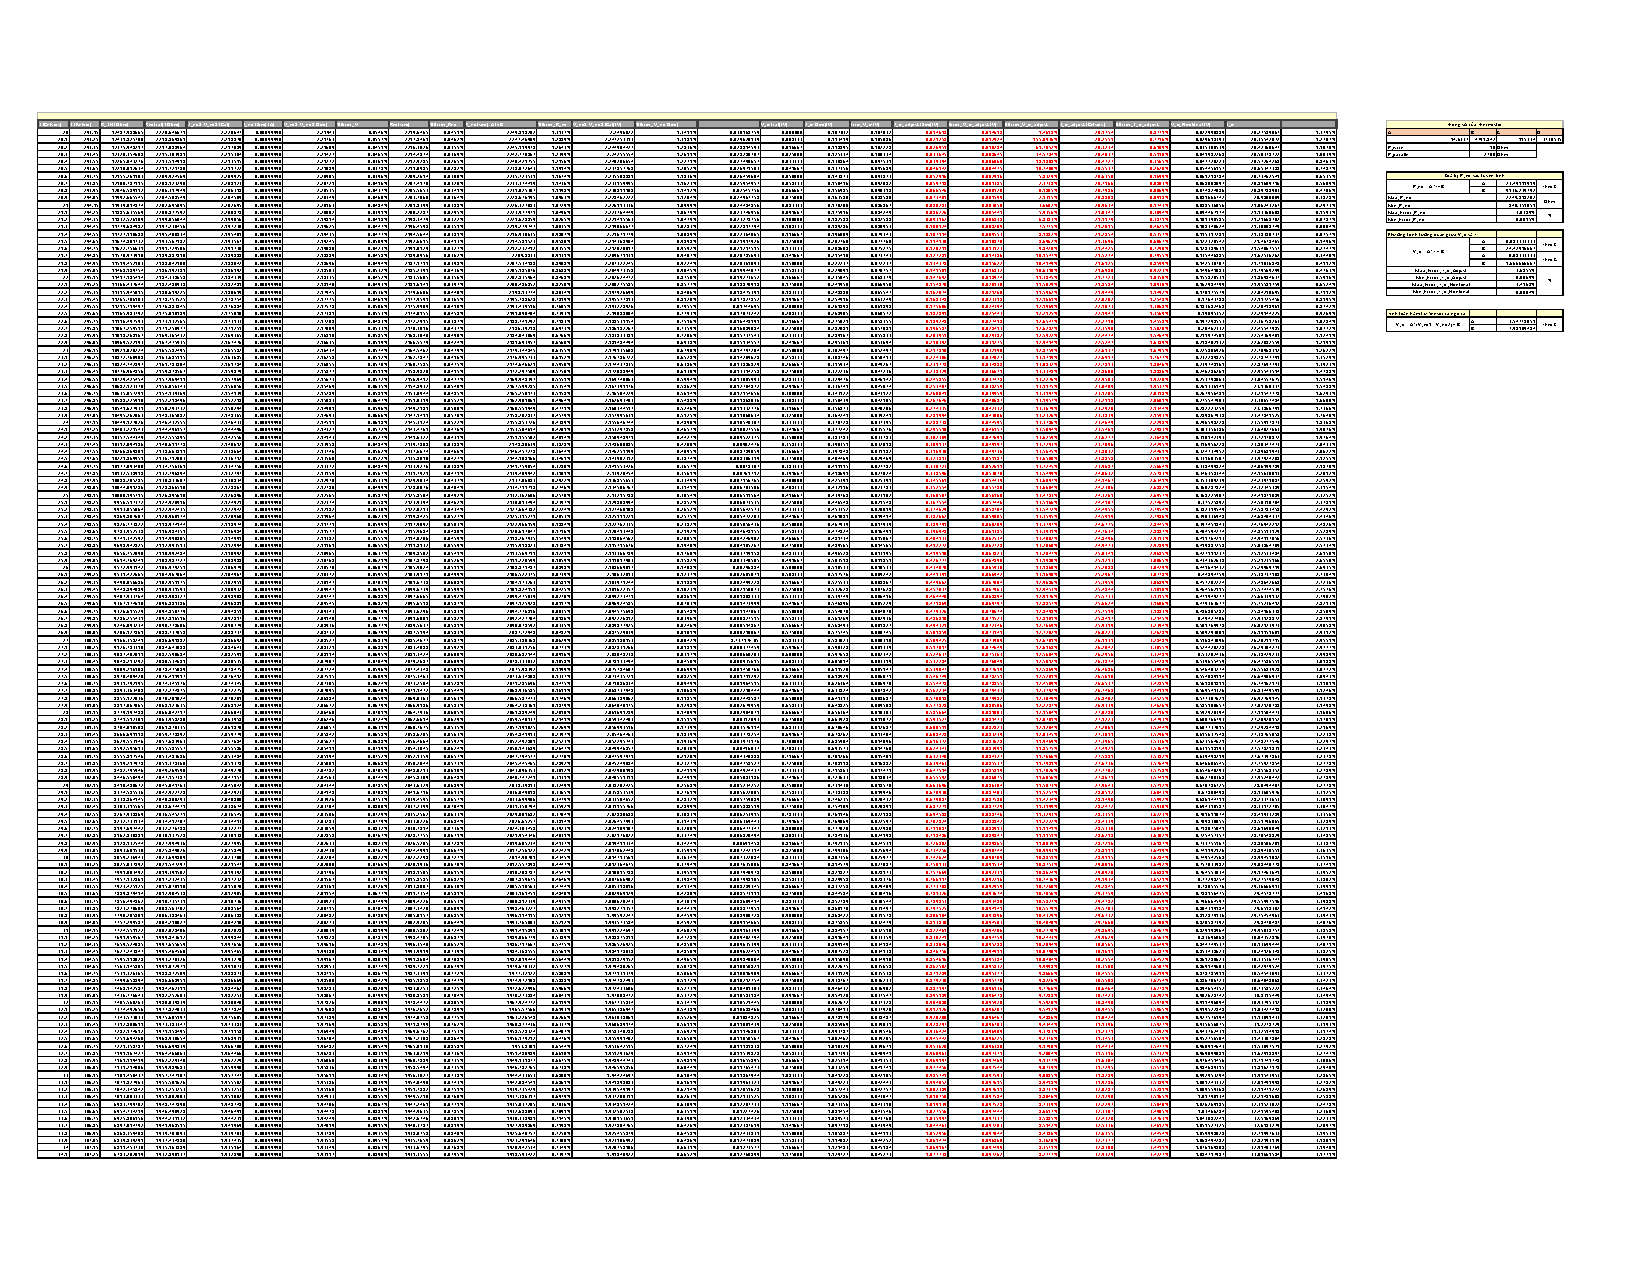
\includepdf[pages=-,angle=90,offset=0cm 0cm]{./my-chapters/my-images/PROJECT.pdf}
\end{landscape}